%documentclass[pdftex,10pt,a4paper,oneside]{book}
%Can change the pt, papersize etc.
\documentclass[oneside]{book}
\usepackage{blindtext}
\usepackage[T1]{fontenc}
\usepackage[utf8]{inputenc}
% \usepackage{algorithm}
% \usepackage{algorithmic} %Algorithm styles, need to be nested for the example shown
\usepackage{fancyhdr} %For our headers
\usepackage{graphicx} %Inserting images
\usepackage{lipsum}  %Blank text fill, delete me when finished
\usepackage{setspace} %Spacing on the front page for crest and titles
\usepackage[]{fncychap} % Styles can be Sonny, Lenny, Glenn, Conny, Rejne, Bjarne and Bjornstrup
\usepackage[hyphens]{url} %Deals with hyphens in urls to make them clickable
\usepackage{xcolor} %Great if you want coloured text
\usepackage{tabularx}
\usepackage{appendix} %Take a wild guess slick

%KEEP THIS ONE LAST it's quite buggy, it allows you to click on links within the pdf and web links without changing the colour. The mouse cursor simply changes its icon to indicate to the user. Great tool - still awkward
\usepackage[hidelinks]{hyperref}


%This will tell the compiler to do the header style, page and spacing between the header and text
\fancyhf{}
\renewcommand{\headrulewidth}{0.2pt}
\newcolumntype{P}[1]{>{\centering\arraybackslash}p{#1}}

\usepackage{float} 
\usepackage{import}
\graphicspath{ {figures/} }
\usepackage{array}
\usepackage{xcolor,colortbl}
\definecolor{Gray}{gray}{0.85}


\usepackage{tabularx}
    \newcolumntype{L}{>{\raggedright\arraybackslash}X}

\usepackage[utf8]{inputenc}
\usepackage{array}
\usepackage{makecell}
\usepackage{array,multirow}

\renewcommand\theadalign{bc}
\renewcommand\theadfont{\bfseries}
\renewcommand\theadgape{\Gape[4pt]}
\renewcommand\cellgape{\Gape[4pt]}
 

\newtheorem{defn}{Definition}[section]
\title{Image and video retreival system}
\author{Multimedia team}
\date{May 2021}
% Specification
\usepackage[utf8]{inputenc}
\usepackage{array}
\usepackage{makecell}
\usepackage{array,multirow}

\renewcommand\theadalign{bc}
% for \\ PCIe Physical Layer\\

\begin{document}


\thispagestyle{empty}

\begin{spacing}{1}
	\begin{center}
		
\includegraphics[scale = 0.20]{Images/ASU.png}
	\end{center}
	\vspace{10mm}
	\begin{center}
		\textbf{\begin{LARGE}
		Image And Video Retreival System
		\end{LARGE}}
		
	\end{center}
% 	\begin{center}
% 		{\large Research proficiency exam}\\
% 		\vspace{20mm}
% 	\end{center}
	\begin{center}
		\textbf{\large Mohammed Emad Mahmoud\\ Mohamed Hussien Mostafa \\ Mohamed Ahmed Abd Alazeem
		\\Mohamed Amr Mohamed\\Mohamed Amr Ahmed\\Mohamed Khaled Mohamed\\Mohamed khaled rashad\\Mohamed gamal Talaat}
		\vspace{30mm}
	\end{center}
	\begin{center}
	     {\large Supervisor: Dr.Gamal A. Ebrahim}\\
		\textbf{\large Department of Computer Systems Engineering}\\
		{\large Faculty of Engineering at Ain Shams University}\\
		{\large May 2021\\}
	\end{center}
\end{spacing}

\pagenumbering{roman}

\pagenumbering{arabic}

\tableofcontents
\listoffigures
\listoftables
\pagebreak
\chapter{Introduction}
The quantity of virtual content, withinside the shape of snap shots
and video, has been growing exponentially in current years.
With growing computing strength and digital storage
capacity, the capability for big virtual photo/video libraries is
developing rapidly. In particular, the World Wide Web has seen
an expanded use of virtual snap shots and video, which shape
the bottom of many entertainment, educational, and commercial
applications. As a result, it has grow to be extra and extra
difficult for a consumer to look for the applicable records
amongst a big quantity of virtual snap shots or video. Image
and video libraries consequently want to offer smooth informational get entry to and the retrieval records ought to be smooth to
locate, manipulate and display.
As the dimensions of reachable photo and video collections
grows to lots of hours, capability visitors will want
abstractions and era that assist them browse effectively
and efficiently. Text-primarily based totally seek algorithms provide some
help in locating precise snap shots or segments amongst
big video collections. In maximum cases, however, those systems
output many beside the point snap shots or video segments to ensure
retrieval of pertinent records. Intelligent indexing systems
are crucial for gold standard retrieval of photo and video data.
A standard content-primarily based totally photo/video retrieval gadget
consists of 3 principal aspects: characteristic extraction, excessive dimensional indexing and gadget layout [24]. Among the 3
aspects, excessive dimensional indexing is vital for speed
overall performance; gadget layout is crucial for look overall performance; and characteristic extraction is the important thing to accuracy overall performance. The accuracy overall performance of a retrieval gadget is
very subjective and consumer-dependent. To a consumer, the similarity
among items is frequently excessive-degree or semantic. However,
capabilities we are able to extract from items are frequently low-degree
capabilities, as maximum of them are extracted immediately from virtual
representations of items withinside the database. The hole among
low-degree capabilities and excessive-degree semantics has been the
principal impediment to higher retrieval overall performance.
In this bankruptcy we discover the today's technology in
photo and video retrieval. We describe numerous techniques for
extracting capabilities which can be used to degree photo and video
similarity in multimedia databases. We additionally describe strategies to bridge the space among low-degree capabilities and
excessive-degree semantics.
\chapter{Project Description}
\section{Detailed project description}
%Begin from here





\section{Beneficiaries of the project}
%Begin from here





\section{Detailed analysis}
%Begin from here




\section{Techniques description}
\subsection{Images techniques}

\subsubsection{Mean color}
This technique depends on computing the distance between images based on the color similarity between them. 
For RGB images the mean color of pixels is computed by finding the average color of the pixels in each channel 
separately then finding the average between the three
values that result from each channel. To get the most similar images to the input image ,the difference between the mean color the input image 
and each image in the database is computed then we apply a reasonable threshold to execlude the images with large distance.
\vskip 0.2in
Mean color is one of the most techniques used in image retreival systems 
because it can be completed without regard to image size or orientation and it needs less computational power than other techniques.


\subsubsection{Histogram}
Histogram search algorithms , characterize an image by its
color distribution or histogram. A histogram is nothing but
a graph that represents all the colors and the level of their
occurrence in an image irrespective of the type of the
image. 
\vskip 0.2in
Few basic properties about an image can be obtained
from using a Histogram. It can be used to set a threshold for
screening the images. The shape and the concentration of
the colors in the histogram will be the same for similar
objects even though they are of different colors.
\vskip 0.2in
Identifying objects in a grey scale image is the easiest one as the
histogram is almost similar as the objects have the same
colors for same objects. In order for identifying the objects
in the images or generating the histogram the system has to
obtain the array values of the frequency of occurrence of each color value -from 0 to 255- in the image.
\vskip 0.2in

\begin{figure}[H]
    \centering
    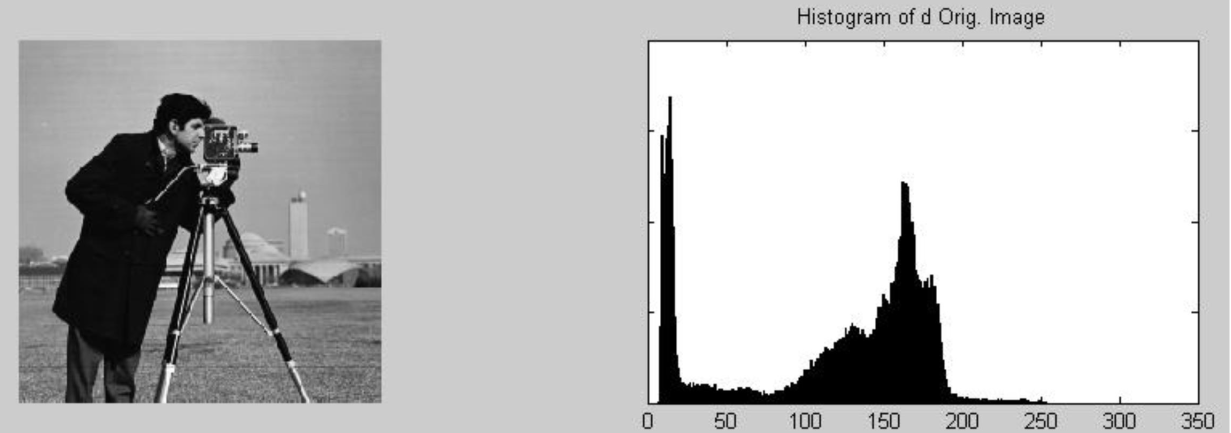
\includegraphics[width=70mm,height=40mm]{Images/hist.png}
    \caption{example for image histogram}
  \end{figure}
\vskip 0.2in

To calculate the distance between two image histogram we calculate the sum of the
smallest bin for each corresponding bins in the two histograms
for input image I and the model image M normalized to the
number of pixels in the model image.
\vskip 0.2in

\begin{figure}[H]
    \centering
    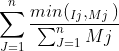
\includegraphics[width=40mm,height=20mm]{Images/eq.png}
    \caption{histogram distance equation}
  \end{figure}

  \vskip 0.2in
\subsubsection{Color Layout}
This technique is similar to histogram based technique except it solves the problem of getting results of images with a low 
histogram distance value but with a different contents.
\vskip 0.2in
In this algorithm we divide each image into 5x5 array of blocks so we get 25 sub-image then we calculate the histogram form each block.
To find the distance between to images we get the distance between the histograms of each two corresponding block, 
then we calculate the total distance by finding the summation of all blocks distance.
\vskip 0.2in

\begin{figure}[H]
    \centering
    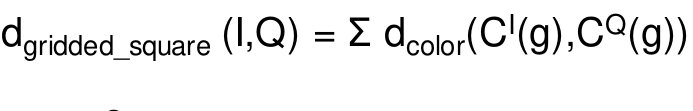
\includegraphics[width=80mm,height=20mm]{Images/cl.png}
    \caption{color layout distance equation}
  \end{figure}
  
  \vskip 0.2in

\subsection{Videos techniques}
%Begin from here
\subsubsection{Feature extraction technique}
\vskip 0.2in
To make a content based video retrieval system, we have to deal with videos as frames and compare frame with each others as images.
But applying this technique would consume a lot of memory to store the whole frame of each video.
So the key frames role appear here.
\vskip 0.2in
A key frame (or keyframe) in animation and filmmaking is a drawing or shot that defines the starting 
and ending points of any smooth transition. These are called frames because their position in time is measured in 
frames on a strip of film or on a digital video editing timeline.
\vskip 0.2in
So we make a key frame extraction operation for each video before inserting it to the database.
then we deal with key frames as the same manners of images, We caculate the histogram for each key frame and divide the range into 
five regions then we get the averge of each region resulting the five values that we store in the data base, after that we use these values
as a initial filtering to get the most similar frames of the input ,then we use the accurate -255 values- histogram to make a second step filtering.
\vskip 0.2in
\subsubsection{Distance calculation}
To get the distance between two videos we use the naive video similarity technique.
In this technique we calculate how many key frames in the query video is similar to one or more key frame in the model video, then 
we calculate the ration between these key frames to the total number of the key frames, after that we compare the distance with a threshold valueand if the 
distance is lower than this threshold, the two videos are similar otherwise they are not similar.
\chapter{Project planning}


\section{Task breakdown structure}
%Begin from here

\begin{figure}[H]
    \centering
    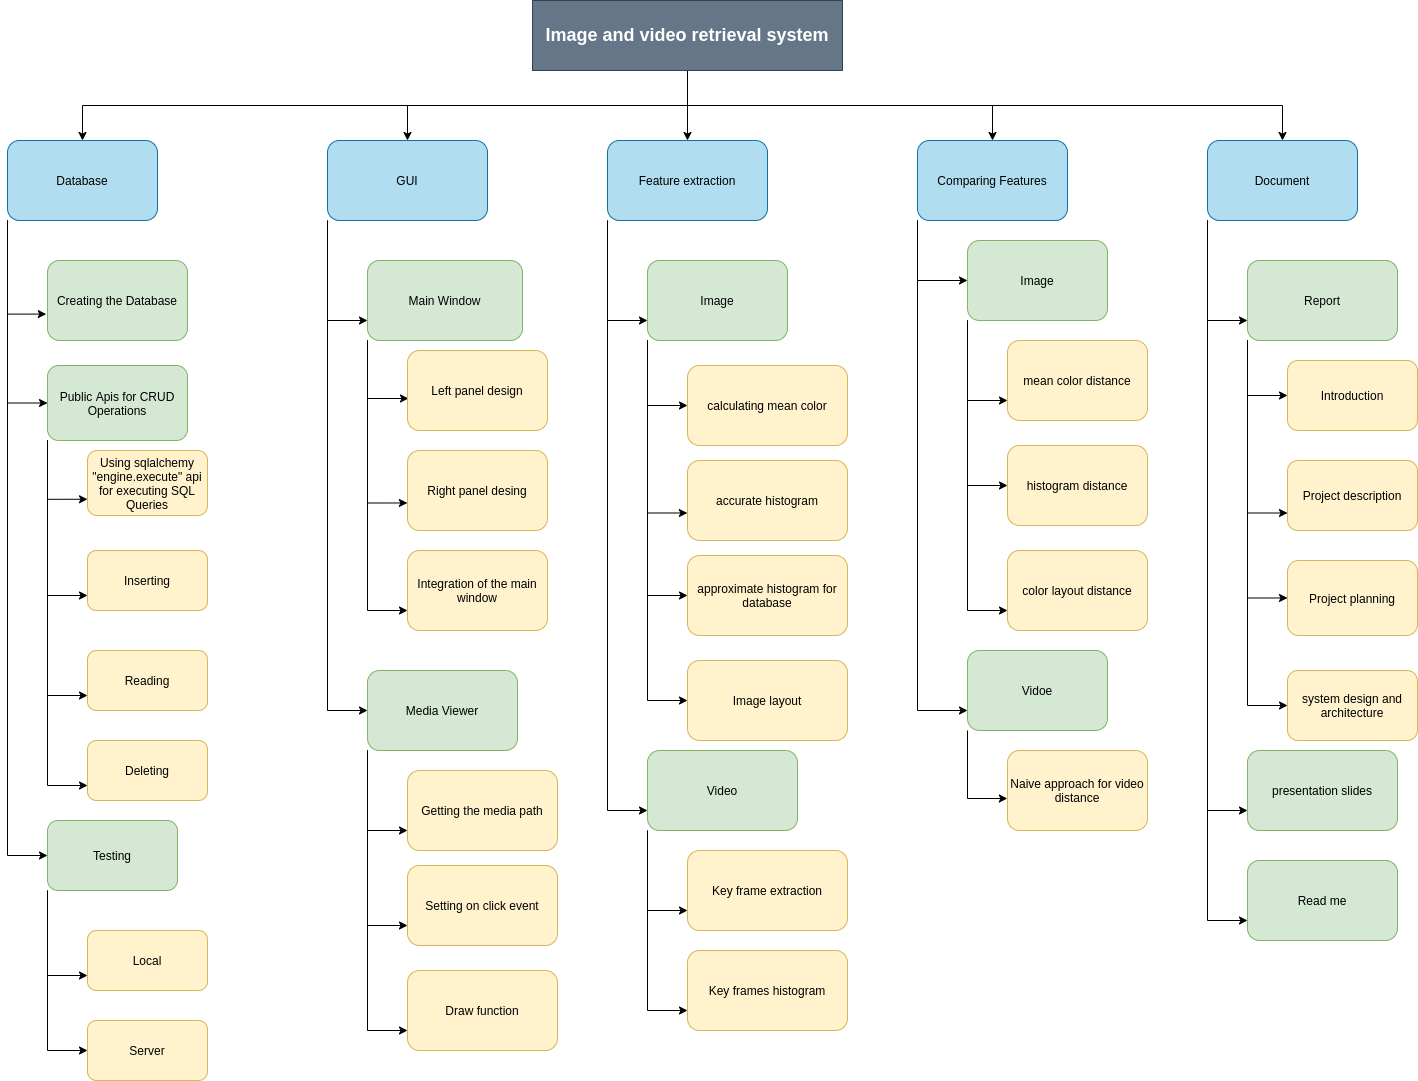
\includegraphics[width=120mm,height=100mm]{Images/TBDS.png}
    \caption{Tasks break down structure}
  \end{figure}




\section{Time plan and Gant chart}
%Begin from here

Firstly, we split all project team members into 3 basic groups in according to simplify the overall problem into 
smaller ones that we can deal with.
We decided to start with designing the database and find best modelling ways to fit our storage requirements.
The second group mission is to implement software functions that do the following:
\vskip 0.2in
\begin{enumerate}
    \item extract data from videos/images.
    \item store the different representations of input data into the database.
    \item impelemnt the required techinques that fit project targets.
\end{enumerate}
According to third group, it provides the project with a well-interactive graphical user interface.
Finally, the last group provides the project full documentation.
\vskip 0.2in
We divided our team into the following:
\begin{enumerate}
    \item Mohammed Khaled Rashad and Mohammed Hussien.
    \item Mohamed Amr Ahmed, Mohamed Amr Mohamed, Mohamed Khaled \vskip 0.05in
     Elkhawas and Mohamed Ahmed Abdel Azem.
    \item Mohammed Gamal Talaat and Mohammed Emad.
    \item Mohammed Hussien Mostafa, Mohammed Ahmed Abd el Azeem and Mohammed Emad.
\end{enumerate}


\begin{figure}[H]
  \centering
  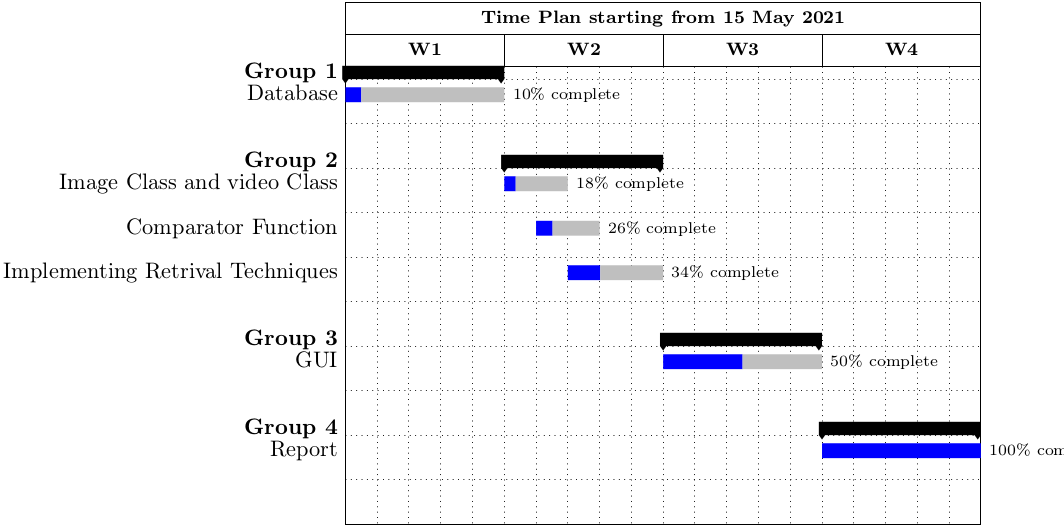
\includegraphics[width=120mm,height=90mm]{Images/time_plan.png}
  \caption{Time Plan starting from 15 May 2021}
\end{figure}
\vskip 0.2in
\end{document}
